 % LuaLaTeX文書; 文字コーAドはUTF-8
 \documentclass[unicode,12pt, A4j]{ltjsarticle}% 'unicode'が必要
 %\usepackage{luatexja}% 日本語したい
 \usepackage{luatexja-fontspec}
 %\usepackage[hiragino-pron]{luatexja-preset}% IPAexフォントしたい(ipaex)
 \usepackage[hiragino-pron,deluxe,expert,bold]{luatexja-preset}
\usepackage{tikz}
\usetikzlibrary{arrows.meta}
\usetikzlibrary{calc}
\usepackage{geometry}
\usepackage{ifthen}
 \usepackage[english]{babel}%多言語文書を作成する
 \usepackage{amsmath,amssymb}%標準数式表現を拡大する
 \usepackage{physics}
 \usepackage[subpreambles=true,sort=true]{standalone}
% \renewcommand{\kanjifamilydefault}{\gtdefault}% 既定をゴシック体に

 \usepackage{mhchem}
 % あとは欧文の場合と同じ




  \usepackage{caption}
  \usepackage[subrefformat=parens]{subcaption}
\title{東大数学理科後期2001年度}
\author{}
\date{}

\begin{document}
\maketitle

\section{問題1}
任意の自然数 $n \ge 2$ に対して,常に不等式
\begin{align}
 n - \sum_{k=2}^{n} \frac{k}{\sqrt{k^2 - 1}} \ge \frac{i}{10}
\end{align}
が成立するような最大の整数 $i$ を求めよ.


\section{問題2}
\begin{enumerate}
    \item 図 1 のように,等間隔 $h$ で格子状に互いに直交する 2 組の無限の平行線が引いてある平面が与えられている.その上に半径 1 の円 $C$ を無作為に落とすとき,この円 $C$ がちょうど 2 本の線と交わる確率 $p$ を求めよ.
    \item 図 2 のように,半径 $\sqrt{2} + 1$ の円が重複なく,かつ隣り合う円と接して無限に敷き詰められた平面がある.この上に半径 1 の円 $C$ を無作為に落とすとき,その円 $C$ が平面上のちょうど 3 つの円と交わる確率 $q$ を求めよ.ただし,解答にあたり次のことを用いてよい.

    平面上に共に始点 $O$ を始点とする一次独立な 2 つのベクトル $\mathbf{a}, \mathbf{b}$ を考え,点 $O$ と $\mathbf{a}, \mathbf{b}, \mathbf{a} + \mathbf{b}$ の 3 つのベクトルの終点の 4 点を頂点とする平行四辺形を $E$ とする.$E$ の領域 $F$ に対して,$\mathbf{f} \in F$ を $\mathbf{a}$ と $\mathbf{b}$ の整数係数の一時結合 $m\mathbf{a} + n\mathbf{b}$ によって平行移動したものの全体を $D$ とする.即ち記号で書くと
    \begin{align}
         D = \{\mathbf{x} + m\mathbf{a} + n\mathbf{b} \mid \mathbf{x} \in F, m \in \mathbb{Z}, n \in \mathbb{Z} \}
    \end{align}
    とおく.ここで $\mathbb{Z}$ は整数全体の集合を表す.

    このとき平面に 1 点を無作為に落とすとき,その点が $D$ に落ちる確率は,平行四辺形 $E$ の面積に対する領域 $F$ の面積の比になっている.
\end{enumerate}

    \begin{figure}[h]
     \centering
        \tikzset{
            % axis/.style={very thick, ->, >=stealth'},
            dashed_line/.style={dashed, thin},
        }
        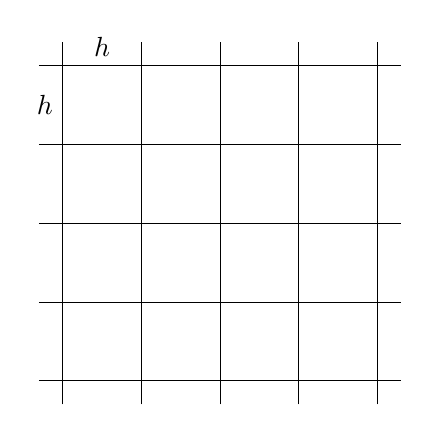
\begin{tikzpicture}
	 \foreach \i in {0,...,4} {
	 % Horizontal lines
	 \draw (-0.3, {\i}) -- (4.3, {\i});
	 \draw ({\i}, -0.3) -- ({\i}, 4.3);

	 }
	 \coordinate (A) at (0.5,4.0);
	 \node[above] at (A) {$h$};
	 \coordinate (B) at (0,3.5);
	 \node[left] at (B) {$h$};
        \end{tikzpicture}
     \caption{図1}
    \end{figure}

    \begin{figure}[h]
     \centering
        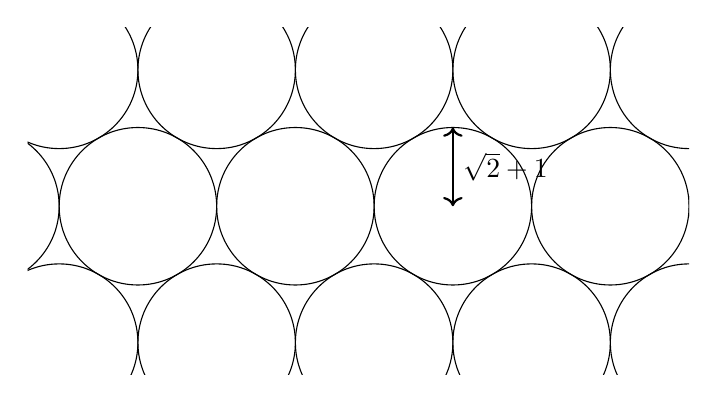
\begin{tikzpicture}
	 \clip (-0.4,-0.4) rectangle (8,4);

	 \foreach \i in {-2,...,5} {
	 \draw[circle] ({2*\i}, 0 ) circle (1);
	 \draw[circle] ({2*\i}, {2*sqrt(3)} ) circle (1);
	 \draw[circle] ({2*\i+1}, {sqrt(3)} ) circle (1);
	 }
	 
	 \draw[thick, <->] (5,{sqrt(3)}) -- (5,{sqrt(3)+1}) node[midway, right] {$\sqrt{2}+1$};
	\end{tikzpicture}
     \caption{図2}

    \end{figure}


\section{問題3}
整数を係数とする 2 次方程式 $f(x)$ で 2 次の項の係数が正であるものが与えられている.任意の正の実数 $x$ に対して,平面の原点を中心とし半径が 1 である単位円 $C$ 上の点 $P(x)$ を
\[
P(x) = (\cos 2\pi f(x), \sin 2\pi f(x))
\]
によって定める.円周 $C$ の弧 $I$ の長さが $L$ ($0 < L < 2\pi$) であるものを固定する.このとき各自然数 $k$ に対して区間 $[k, k+1]$ の部分集合
\[
\{x \mid k \le x \le k+1, P(x) \in I \}
\]
は互いに交わらない有限個の閉区間の和集合になっているので,それらの区間の長さの総和を $T_k$ で表す.このとき,$\lim_{k \to \infty} T_k = \frac{L}{2\pi}$ を証明せよ.

\end{document}